% \iffalse meta-comment
%
% Copyright (C) 2015 by Josef Friedrich <josef@friedrich.rocks>
% ----------------------------------------------------------------------
% This work may be distributed and/or modified under the conditions of
% the LaTeX Project Public License, either version 1.3 of this license
% or (at your option) any later version.  The latest version of this
% license is in:
%
%   http://www.latex-project.org/lppl.txt
%
% and version 1.3 or later is part of all distributions of LaTeX
% version 2005/12/01 or later.
%
% This work has the LPPL maintenance status `maintained'.
%
% The Current Maintainer of this work is Josef Friedrich.
%
% This work consists of the files nodetree.dtx and nodetree.ins
% and the derived filebase nodetree.sty and nodetree.lua.
%
% \fi
%
% \iffalse
%<*driver>
\ProvidesFile{nodetree.dtx}
%</driver>
%<package>\NeedsTeXFormat{LaTeX2e}[1999/12/01]
%<package>\ProvidesPackage{nodetree}
%<*package>
    [2015/11/13 Package to debug node lists used by LuaTeX]
%</package>
%<*driver>
\documentclass{ltxdoc}
\usepackage{paralist,fontspec,graphicx,fancyvrb}
\usepackage[
  colorlinks=true,
  linkcolor=red,
  filecolor=red,
  urlcolor=red,
]{hyperref}
\EnableCrossrefs
\CodelineIndex
\RecordChanges

\setmonofont{DejaVu Sans Mono}

\def\nodetreelua#1{\texttt{\scantokens{\catcode`\_=12\relax#1}}}

\def\secref#1{(\rightarrow\ \ref{#1})}

\DefineVerbatimEnvironment{code}{Verbatim}
{
  frame=single,
  fontsize=\footnotesize,
  numbers=left,
  numbersep=2mm,
}

\begin{document}

\providecommand*{\url}{\texttt}
\GetFileInfo{nodetree.dtx}
\title{The \textsf{nodetree} package}
\author{%
  Josef Friedrich\\%
  \url{josef@friedrich.rocks}\\%
  \href{https://github.com/Josef-Friedrich/cloze}{github.com/Josef-Friedrich/nodetree}%
}
\date{\fileversion~from \filedate}

\maketitle

\noindent
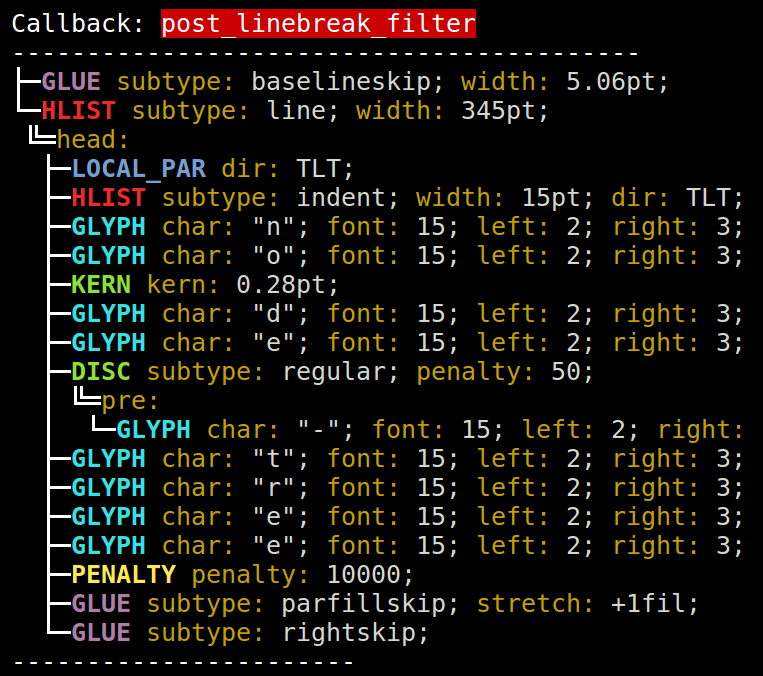
\includegraphics[width=\linewidth]{graphics/nodetree}

\newpage

\tableofcontents

\newpage

\section{Abstract}

|nodetree| is a development package that visualizes the structure of
node lists in a tree view. Node lists are the main building blocks of
each document generated by the \TeX{} engine \emph{Lua\TeX}. The nodes
are displayed in a tree view similar to the UNIX |tree| command. The
package |nodetree| doesn‘t change the rendered document. The tree view
can only be seen when using a terminal to generate the document.

\section{Usage}

The package |nodetree| can be used both with Lua\TeX and Lua\LaTeX. You
have to use both engines in a text console. Run |luatex luatex-test.tex|
for example to list the nodes using Lua\TeX.

\begin{code}
%%
%% This is file `nodetree.tex',
%% generated with the docstrip utility.
%%
%% The original source files were:
%%
%% nodetree.dtx  (with options: `tex')
%% 
%% This is a generated file.
%% 
%% Copyright (C) 2015 by Josef Friedrich <josef@friedrich.rocks>
%% ----------------------------------------------------------------------
%% This work may be distributed and/or modified under the conditions of
%% the LaTeX Project Public License, either version 1.3c of this license
%% or (at your option) any later version. The latest version of this
%% license is in:
%% 
%%   http://www.latex-project.org/lppl.txt
%% 
%% and version 1.3c or later is part of all distributions of LaTeX
%% version 2008/05/05 or later.
%% 
\directlua{
  nodetree = require('nodetree')
  nodetree.set_option('engine', 'luatex')
}
\def\nodetreeoption[#1]#2{
  \directlua{
    nodetree.set_option('#1', '#2')
  }
}
\endinput
%%
%% End of file `nodetree.tex'.

\nodetreeregister{linefilter}

Lorem ipsum dolor.
\bye
\end{code}

Or run |lualatex lualatex-test.tex| to show a node tree using Lua\LaTeX.

\begin{code}
\documentclass{article}
\usepackage[callback=linefilter]{nodetree}

\begin{document}
Lorem ipsum dolor.
\end{document}
\end{code}

\subsection{Debug nodes inside Lua code}

Use the Lua function |nodetree.analyze(head)| to debug nodes inside your
Lua code. The following code snippet demonstrates the usage in Lua\TeX.
|head| is the current node.

\begin{code}
%%
%% This is file `nodetree.tex',
%% generated with the docstrip utility.
%%
%% The original source files were:
%%
%% nodetree.dtx  (with options: `tex')
%% 
%% This is a generated file.
%% 
%% Copyright (C) 2015 by Josef Friedrich <josef@friedrich.rocks>
%% ----------------------------------------------------------------------
%% This work may be distributed and/or modified under the conditions of
%% the LaTeX Project Public License, either version 1.3c of this license
%% or (at your option) any later version. The latest version of this
%% license is in:
%% 
%%   http://www.latex-project.org/lppl.txt
%% 
%% and version 1.3c or later is part of all distributions of LaTeX
%% version 2008/05/05 or later.
%% 
\directlua{
  nodetree = require('nodetree')
  nodetree.set_option('engine', 'luatex')
}
\def\nodetreeoption[#1]#2{
  \directlua{
    nodetree.set_option('#1', '#2')
  }
}
\endinput
%%
%% End of file `nodetree.tex'.


\directlua{
  local test = function (head)
    nodetree.analyze(head)
  end
  callback.register('post_linebreak_filter', test)
}

Lorem ipsum dolor.
\bye
\end{code}

This example illustrates how the function has to be applied in
Lua\LaTeX.

\begin{code}
\documentclass{article}
\usepackage{nodetree}

\begin{document}

\directlua{
  local test = function (head)
    nodetree.analyze(head)
  end
  luatexbase.add_to_callback('post_linebreak_filter', test, 'test')
}

Lorem ipsum dolor.
\end{document}
\end{code}

%-----------------------------------------------------------------------
%
%-----------------------------------------------------------------------

\section{Macros}

%%
% \nodetreeregister
%%

\subsection{\cmd{\nodetreeregister}}

\DescribeMacro{\nodetreeregister}
\cmd{\nodetreeregister}\marg{callbacks}: The argument \marg{callbacks}
takes a comma separated list of callback aliases as described in
\secref{sec:option-callback}.

%%
% \nodetreeunregister
%%

\subsection{\cmd{\nodetreeunregister}}

\DescribeMacro{\nodetreeunregister}
\cmd{\nodetreeunregister}\marg{callbacks}: The argument \marg{callbacks}
takes a comma separated list of callback aliases as described in
\secref{sec:option-callback}.

%%
% \nodetreeoption
%%

\subsection{\cmd{\nodetreeoption}}

\DescribeMacro{\nodetreeoption}
\cmd{\nodetreeoption}\oarg{option}\marg{value}: \secref{sec:options}

%%
% \nodetreeset
%%

\subsection{\cmd{\nodetreeset}}

\DescribeMacro{\nodetreeset}
\cmd{\nodetreeset}\marg{kv-options}:

%-----------------------------------------------------------------------
%
%-----------------------------------------------------------------------

\section{Options}
\label{sec:options}

\subsection{Option \texttt{callback}}
\label{sec:option-callback}

The option |callback| is the most important setting of the package. You
have to specify one alias to select the |callback|. Because of the
underscores the callback name contains it can not set by its technical
name (\rightarrow{} Figure \ref{fig:callback}).

This macros process callback options:
\cmd{\nodetreeregister}\marg{callbacks},
\cmd{\nodetreeunregister}\marg{callbacks},
\cmd{\nodetreeset}\marg{callback=<callbacks>} and
\cmd{\usepackage}\oarg{callback=<callbacks>}\marg{nodetree}.

Use commas to specify mulitple callbacks. Avoid using whitespaces:

\begin{code}
\nodetreeregister{preline,line,postline}
\end{code}

Wrap your callback aliases in curly braces for the macro |\nodetreeset|:

\begin{code}
\nodetreeset{callback={preline,line,postline}}
\end{code}

The same applies for the macro |\usepackage|:

\begin{code}
\usepackage{callback={preline,line,postline}}
\end{code}

%%
%
%%


\newcommand{\nodetreecallback}[3]{
  \nodetreelua{#1} & \nodetreelua{#2} & \nodetreelua{#3} \\
}

\begin{figure}

\noindent
\begin{tabular}{lll}
\textbf{Alias 1} & \textbf{Alias 2} & \textbf{Callback} \\
\nodetreecallback{contribute}{contributefilter}{contribute_filter}
\nodetreecallback{buildpage}{buildpagefilter}{buildpage_filter}
\nodetreecallback{preline}{prelinebreakfilter}{pre_linebreak_filter}
\nodetreecallback{line}{linebreakfilter}{linebreak_filter}
\nodetreecallback{append}{appendtovlistfilter}{append_to_vlist_filter}
\nodetreecallback{postline}{postlinebreakfilter}{post_linebreak_filter}
\nodetreecallback{hpack}{hpackfilter}{hpack_filter}
\nodetreecallback{vpack}{vpackfilter}{vpack_filter}
%\nodetreecallback{hpackq}{hpackquality}{hpack_quality}
%\nodetreecallback{vpackq}{vpackquality}{vpack_quality}
\nodetreecallback{process}{processrule}{process_rule}
\nodetreecallback{preout}{preoutputfilter}{pre_output_filter}
\nodetreecallback{hyph}{hyphenate}{hyphenate}
\nodetreecallback{liga}{ligaturing}{ligaturing}
\nodetreecallback{kern}{kerning}{kerning}
\nodetreecallback{insert}{insertlocalpar}{insert_local_par}
\nodetreecallback{mhlist}{mlisttohlist}{mlist_to_hlist}
\end{tabular}

\caption{The callback aliases}
\label{fig:callback}
\end{figure}

\subsection{Option \texttt{verbosity}}

\subsection{Option \texttt{color}}

\subsection{Option \texttt{decimalplaces}}

\section{Visual tree structure}

\subsection{Two different connections}

Nodes in Lua\TeX are connected. The |nodetree| package distinguishs
between the |list| and |field| connections.

\begin{itemize}
 \item |list|: Nodes, which are double connected by |next| and
       |previous| fields.
 \item |field|: Connections to nodes by other fields than |next| and
       |previous| fields, e. g. |head|, |pre|.
\end{itemize}

\subsection{Unicode characters to show the tree view}

\renewcommand{\arraystretch}{1.5}

The package |nodetree| uses the unicode box drawing symbols. Your
default terminal font should contain this characters to obtain the tree
view. Eight box drawing characters are necessary.

\noindent
\begin{tabular}{lcl}
\textbf{Code} & \textbf{Character} & \textbf{Name} \\
U+2500 & |─| & BOX DRAWINGS LIGHT HORIZONTAL \\
U+2502 & |│| & BOX DRAWINGS LIGHT VERTICAL \\
U+2514 & |└| & BOX DRAWINGS LIGHT UP AND RIGHT \\
U+251C & |├| & BOX DRAWINGS LIGHT VERTICAL AND RIGHT \\
U+2550 & |═| & BOX DRAWINGS DOUBLE HORIZONTAL \\
U+2551 & |║| & BOX DRAWINGS DOUBLE VERTICAL \\
U+255A & |╚| & BOX DRAWINGS DOUBLE UP AND RIGHT \\
U+2560 & |╠| & BOX DRAWINGS DOUBLE VERTICAL AND RIGHT \\
\end{tabular}

For |list| connections \emph{light} characters are shown.

\begin{code}
│ │
│ ├─list1
│ └─list2
└─list3
\end{code}

|field| connections are visialized by \emph{Double} characters.

\begin{code}
║ ║
║ ╠═field1
║ ╚═field2
╚═field3
\end{code}


\section{Example tree views}

\noindent
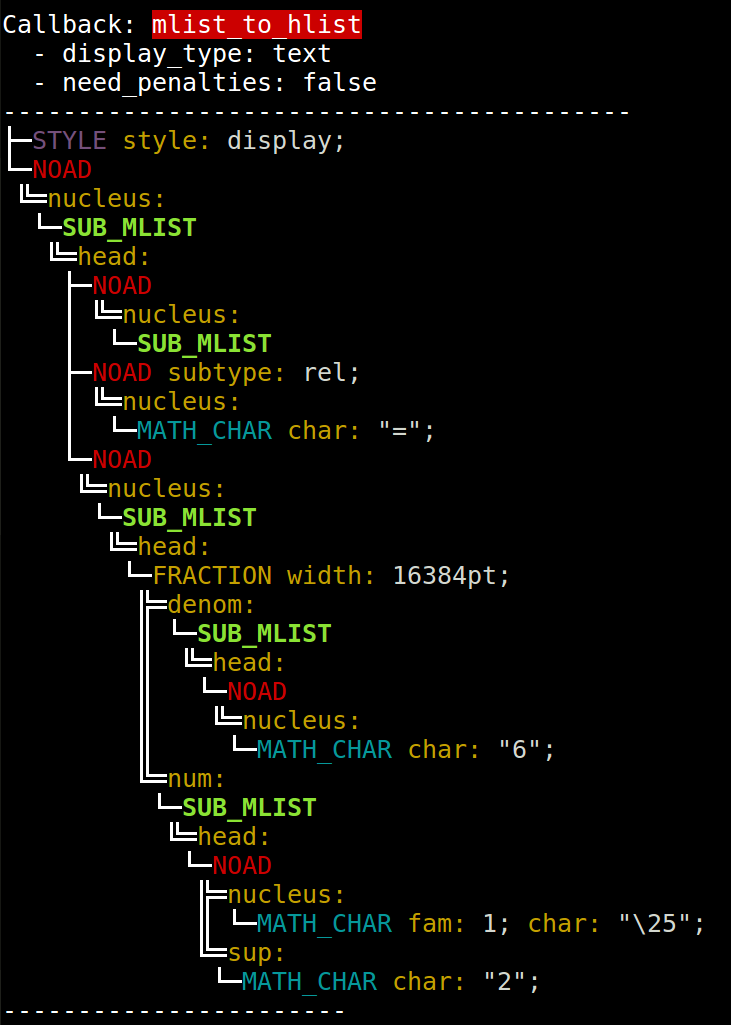
\includegraphics[width=\linewidth]{graphics/mhlist}

  \DocInput{nodetree.dtx}
  \pagebreak
  \PrintChanges
  \pagebreak
  \PrintIndex
\end{document}
%</driver>
%<*readme>
# nodetree

Inspired by a [gist of Patrick Gundlach](https://gist.github.com/pgundlach/556247).

`nodetree` displays some debug informations of the node list in the
terminal, when you render a Latex document.

```
post_linebreak_filter:
│
├─GLUE subtype: baselineskip; width: 5.06pt;
└─HLIST subtype: line; width: 345pt; height: 6.94pt; dir: TLT; glue_order: 2; glue_sign: 1; glue_set: 304.99993896484;
 ╚═head:
  ├─LOCAL_PAR dir: TLT;
  ├─HLIST subtype: indent; width: 15pt; dir: TLT;
  ├─GLYPH char: "O"; font: 15; left: 2; right: 3; uchyph: 1; width: 7.78pt; height: 6.83pt;
  ├─DISC subtype: regular; penalty: 50;
  │ ╠═post:
  │ ║ └─GLYPH subtype: ghost; char: "\12"; font: 15; width: 5.56pt; height: 6.94pt;
  │ ║  ╚═components:
  │ ║   ├─GLYPH subtype: ligature; char: "f"; font: 15; left: 2; right: 3; uchyph: 1; width: 3.06pt; height: 6.94pt;
  │ ║   └─GLYPH subtype: ligature; char: "i"; font: 15; left: 2; right: 3; uchyph: 1; width: 2.78pt; height: 6.68pt;
  │ ╠═pre:
  │ ║ ├─GLYPH char: "f"; font: 15; left: 2; right: 3; uchyph: 1; width: 3.06pt; height: 6.94pt;
  │ ║ └─GLYPH char: "-"; font: 15; left: 2; right: 3; uchyph: 1; width: 3.33pt; height: 4.31pt;
  │ ╚═replace:
  │  └─GLYPH subtype: ghost; char: "\14"; font: 15; width: 8.33pt; height: 6.94pt;
  │   ╚═components:
  │    ├─GLYPH subtype: ghost; char: "\11"; font: 15; width: 5.83pt; height: 6.94pt;
  │    │ ╚═components:
  │    │  ├─GLYPH subtype: ligature; char: "f"; font: 15; left: 2; right: 3; uchyph: 1; width: 3.06pt; height: 6.94pt;
  │    │  └─GLYPH subtype: ligature; char: "f"; font: 15; left: 2; right: 3; uchyph: 1; width: 3.06pt; height: 6.94pt;
  │    └─GLYPH subtype: ligature; char: "i"; font: 15; left: 2; right: 3; uchyph: 1; width: 2.78pt; height: 6.68pt;
  ├─GLYPH char: "c"; font: 15; left: 2; right: 3; uchyph: 1; width: 4.44pt; height: 4.31pt;
  ├─GLYPH char: "e"; font: 15; left: 2; right: 3; uchyph: 1; width: 4.44pt; height: 4.31pt;
  ├─PENALTY penalty: 10000;
  ├─GLUE subtype: parfillskip; stretch: 65536; stretch_order: 2;
  └─GLUE subtype: rightskip;

```

%</readme>
% \fi
%
% \CheckSum{0}
%
% \CharacterTable
%  {Upper-case    \A\B\C\D\E\F\G\H\I\J\K\L\M\N\O\P\Q\R\S\T\U\V\W\X\Y\Z
%   Lower-case    \a\b\c\d\e\f\g\h\i\j\k\l\m\n\o\p\q\r\s\t\u\v\w\x\y\z
%   Digits        \0\1\2\3\4\5\6\7\8\9
%   Exclamation   \!     Double quote  \"     Hash (number) \#
%   Dollar        \$     Percent       \%     Ampersand     \&
%   Acute accent  \'     Left paren    \(     Right paren   \)
%   Asterisk      \*     Plus          \+     Comma         \,
%   Minus         \-     Point         \.     Solidus       \/
%   Colon         \:     Semicolon     \;     Less than     \<
%   Equals        \=     Greater than  \>     Question mark \?
%   Commercial at \@     Left bracket  \[     Backslash     \\
%   Right bracket \]     Circumflex    \^     Underscore    \_
%   Grave accent  \`     Left brace    \{     Vertical bar  \|
%   Right brace   \}     Tilde         \~}
%
%
% \changes{v0.1}{2015/06/16}{Converted to DTX file}
% \changes{v1.0}{2015/07/08}{Inital release}
%
% \DoNotIndex{\newcommand,\newenvironment,\def,\directlua}
%
% \StopEventually{}
% \pagebreak
% \section{Implementation}
%
% \iffalse
%<*tex>
% \fi
% \MacroTopsep = 10pt plus 2pt minus 2pt
% \MacrocodeTopsep = 10pt plus 1.2pt minus 1pt
% \makeatletter
% \c@CodelineNo 25 \relax
% \makeatother
%
% \subsection{The file \tt{nodetree.tex}}
%
%    \begin{macrocode}
\directlua{
  nodetree = require('nodetree')
  nodetree.set_option('engine', 'luatex')
  nodetree.set_default_options()
}
%    \end{macrocode}
%
% \begin{macro}{\nodetreeoption}
%    \begin{macrocode}
\def\nodetreeoption[#1]#2{
  \directlua{
    nodetree.set_option('#1', '#2')
  }
}
%    \end{macrocode}
% \end{macro}
%
% \begin{macro}{\nodetreeregister}
%    \begin{macrocode}
\def\nodetreeregister#1{
  \directlua{
    nodetree.set_option('callback', '#1')
    nodetree.register_callbacks()
  }
}
%    \end{macrocode}
% \end{macro}
%
% \begin{macro}{\nodetreeunregister}
%    \begin{macrocode}
\def\nodetreeunregister#1{
  \directlua{
    nodetree.set_option('callback', '#1')
    nodetree.unregister_callbacks()
  }
}
%    \end{macrocode}
% \end{macro}
%
% \iffalse
%</tex>
%<*package>
% \fi
% \makeatletter
% \c@CodelineNo 25 \relax
% \makeatother
%
% \subsection{The file \tt{nodetree.sty}}
%
%    \begin{macrocode}
%%
%% This is file `nodetree.tex',
%% generated with the docstrip utility.
%%
%% The original source files were:
%%
%% nodetree.dtx  (with options: `tex')
%% 
%% This is a generated file.
%% 
%% Copyright (C) 2015 by Josef Friedrich <josef@friedrich.rocks>
%% ----------------------------------------------------------------------
%% This work may be distributed and/or modified under the conditions of
%% the LaTeX Project Public License, either version 1.3c of this license
%% or (at your option) any later version. The latest version of this
%% license is in:
%% 
%%   http://www.latex-project.org/lppl.txt
%% 
%% and version 1.3c or later is part of all distributions of LaTeX
%% version 2008/05/05 or later.
%% 
\directlua{
  nodetree = require('nodetree')
  nodetree.set_option('engine', 'luatex')
}
\def\nodetreeoption[#1]#2{
  \directlua{
    nodetree.set_option('#1', '#2')
  }
}
\endinput
%%
%% End of file `nodetree.tex'.

\directlua{
  nodetree.set_option('engine', 'lualatex')
}
%    \end{macrocode}
%
%    \begin{macrocode}
\RequirePackage{kvoptions}
%    \end{macrocode}
%
%    \begin{macrocode}
\SetupKeyvalOptions{
  family=NT,
  prefix=NT@
}
%    \end{macrocode}
%
%    \begin{macrocode}
\DeclareStringOption[postlinebreak]{callback}
\define@key{NT}{callback}[]{\nodetreeoption[callback]{#1}}
%    \end{macrocode}
%
%    \begin{macrocode}
\DeclareStringOption[1]{verbosity}
\define@key{NT}{verbosity}[]{\nodetreeoption[verbosity]{#1}}
%    \end{macrocode}
%
%    \begin{macrocode}
\DeclareStringOption[colored]{color}
\define@key{NT}{color}[]{\nodetreeoption[color]{#1}}
%    \end{macrocode}
%
%    \begin{macrocode}
\DeclareStringOption[1]{decimalplaces}
\define@key{NT}{decimalplaces}[]{\nodetreeoption[decimalplaces]{#1}}
%    \end{macrocode}
%
%    \begin{macrocode}
\ProcessKeyvalOptions*
\directlua{
  nodetree.set_default_options()
  nodetree.register_callbacks()
}
%    \end{macrocode}
%
% \begin{macro}{\nodetreeset}
%    \begin{macrocode}
\newcommand{\nodetreeset}[1]{\setkeys{nodetree}{#1}}
%    \end{macrocode}
% \end{macro}
%
% \iffalse
%</package>
%<*luamain>
% \fi
%
% \makeatletter
% \c@CodelineNo 0 \relax
% \makeatother
%
% \subsection{The file \tt{nodetree.lua}}
%
%    \begin{macrocode}
local nodex = {}
%    \end{macrocode}
%
%    \begin{macrocode}
local tpl = {}
%    \end{macrocode}
%
%    \begin{macrocode}
local tree = {}
%    \end{macrocode}
%
% Nodes in Lua\TeX{} are connected. The nodetree view distinguishs
% between the |list| and |field| connections.
%
% \begin{itemize}
%  \item |list|: Nodes, which are double connected by |next| and
%        |previous| fields.
%  \item |field|: Connections to nodes by other fields than |next| and
%        |previous| fields, e. g. |head|, |pre|.
% \end{itemize}
%
% The lua table named |tree.state| holds state values for the current
% tree item.
%
% \begin{code}
%  tree.state:
%    - 1:
%      - list: continue
%      - field: stop
%    - 2:
%      - list: continue
%      - field: stop
% \end{code}
%    \begin{macrocode}
tree.state = {}
%    \end{macrocode}
%
%    \begin{macrocode}
local callbacks = {}
%    \end{macrocode}
%
%    \begin{macrocode}
local base = {}
%    \end{macrocode}
%
%    \begin{macrocode}
local options = {}
%    \end{macrocode}
%
% \subsubsection{nodex --- Extend the node library}
%
% Get the node id form, e. g.:
% \begin{code}
% <node    nil <    172 >    nil : hlist 2>
% \end{code}
%    \begin{macrocode}
function nodex.node_id(n)
  return string.gsub(tostring(n), '^<node%s+%S+%s+<%s+(%d+).*', '%1')
end
%    \end{macrocode}
%
%    \begin{macrocode}
function nodex.subtype(n)
  local typ = node.type(n.id)
  local subtypes = {
%    \end{macrocode}
% \paragraph{hlist (0)}
%    \begin{macrocode}
    hlist = {
      [0] = 'unknown',
      [1] = 'line',
      [2] = 'box',
      [3] = 'indent',
      [4] = 'alignment',
      [5] = 'cell',
      [6] = 'equation',
      [7] = 'equationnumber',
    },
%    \end{macrocode}
% \paragraph{vlist (1)}
%    \begin{macrocode}
    vlist = {
      [0] = 'unknown',
      [4] = 'alignment',
      [5] = 'cell',
    },
%    \end{macrocode}
% \paragraph{rule (2)}
%    \begin{macrocode}
    rule = {
      [0] = 'unknown',
      [1] = 'box',
      [2] = 'image',
      [3] = 'empty',
      [4] = 'user',
    },
%    \end{macrocode}
%
% \noindent
% Nodes without subtypes:
% \begin{compactitem}
% \item ins (3)
% \item mark (4)
% \end{compactitem}
%    \begin{macrocode}
%    \end{macrocode}
% \paragraph{adjust (5)}
%    \begin{macrocode}
    adjust = {
      [0] = 'normal',
      [1] = 'pre',
    },
%    \end{macrocode}
% \paragraph{boundary (6)}
%    \begin{macrocode}
    boundary = {
      [0] = 'cancel',
      [1] = 'user',
      [2] = 'protrusion',
      [3] = 'word',
    },
%    \end{macrocode}
% \paragraph{disc (7)}
%    \begin{macrocode}
    disc  = {
      [0] = 'discretionary',
      [1] = 'explicit',
      [2] = 'automatic',
      [3] = 'regular',
      [4] = 'first',
      [5] = 'second',
    },
%    \end{macrocode}
%
% \noindent
% Nodes without subtypes:
% \begin{compactitem}
% \item whatsit (8)
% \item local\_par (9)
% \item dir (10)
% \end{compactitem}
%
% \paragraph{math (11)}
%    \begin{macrocode}
    math = {
      [0] = 'beginmath',
      [1] = 'endmath',
    },
%    \end{macrocode}
% \paragraph{glue (12)}
%    \begin{macrocode}
    glue = {
      [0]   = 'userskip',
      [1]   = 'lineskip',
      [2]   = 'baselineskip',
      [3]   = 'parskip',
      [4]   = 'abovedisplayskip',
      [5]   = 'belowdisplayskip',
      [6]   = 'abovedisplayshortskip',
      [7]   = 'belowdisplayshortskip',
      [8]   = 'leftskip',
      [9]   = 'rightskip',
      [10]  = 'topskip',
      [11]  = 'splittopskip',
      [12]  = 'tabskip',
      [13]  = 'spaceskip',
      [14]  = 'xspaceskip',
      [15]  = 'parfillskip',
      [16]  = 'mathskip',
      [17]  = 'thinmuskip',
      [18]  = 'medmuskip',
      [19]  = 'thickmuskip',
      [98]  = 'conditionalmathskip',
      [99]  = 'muglue',
      [100] = 'leaders',
      [101] = 'cleaders',
      [102] = 'xleaders',
      [103] = 'gleaders',
    },
%    \end{macrocode}
% \paragraph{kern (13)}
%    \begin{macrocode}
    kern = {
      [0] = 'fontkern',
      [1] = 'userkern',
      [2] = 'accentkern',
      [3] = 'italiccorrection',
    },
%    \end{macrocode}
%
% \noindent
% Nodes without subtypes:
% \begin{compactitem}
% \item penalty (14)
% \item unset (15)
% \item style (16)
% \item choice (17)
% \end{compactitem}
%
% \paragraph{noad (18)}
%    \begin{macrocode}
    noad = {
      [0] = 'ord',
      [1] = 'opdisplaylimits',
      [2] = 'oplimits',
      [3] = 'opnolimits',
      [4] = 'bin',
      [5] = 'rel',
      [6] = 'open',
      [7] = 'close',
      [8] = 'punct',
      [9] = 'inner',
      [10] = 'under',
      [11] = 'over',
      [12] = 'vcenter',
    },
%    \end{macrocode}
% \paragraph{radical (19)}
%    \begin{macrocode}
    radical = {
      [0] = 'radical',
      [1] = 'uradical',
      [2] = 'uroot',
      [3] = 'uunderdelimiter',
      [4] = 'uoverdelimiter',
      [5] = 'udelimiterunder',
      [6] = 'udelimiterover',
    },
%    \end{macrocode}
%
% \noindent
% Nodes without subtypes:
% \begin{compactitem}
% \item fraction (20)
% \end{compactitem}
%
% \paragraph{accent (21)}
%    \begin{macrocode}
    accent = {
      [0] = 'bothflexible',
      [1] = 'fixedtop',
      [2] = 'fixedbottom',
      [3] = 'fixedboth',
    },
%    \end{macrocode}
% \paragraph{fence (22)}
%    \begin{macrocode}
    fence = {
      [0] = 'unset',
      [1] = 'left',
      [2] = 'middle',
      [3] = 'right',
    },
%    \end{macrocode}
%
% \noindent
% Nodes without subtypes:
% \begin{compactitem}
% \item math\_char (23)
% \item sub\_box (24)
% \item sub\_mlist (25)
% \item math\_text\_char (26)
% \item delim (27)
% \item margin\_kern (28)
% \end{compactitem}
%
% \paragraph{glyph (29)}
%    \begin{macrocode}
    glyph = {
      [0] = 'character',
      [1] = 'ligature',
      [2] = 'ghost',
      [3] = 'left',
      [4] = 'right',
    },
%    \end{macrocode}
%
% \noindent
% Nodes without subtypes:
% \begin{compactitem}
% \item align\_record (30)
% \item pseudo\_file (31)
% \item pseudo\_line (32)
% \item page\_insert (33)
% \item split\_insert (34)
% \item expr\_stack (35)
% \item nested\_list (36)
% \item span (37)
% \item attribute (38)
% \item glue\_spec (39)
% \item attribute\_list (40)
% \item temp (41)
% \item align\_stack (42)
% \item movement\_stack (43)
% \item if\_stack (44)
% \item unhyphenated (45)
% \item hyphenated (46)
% \item delta (47)
% \item passive (48)
% \item shape (49)
% \end{compactitem}
%    \begin{macrocode}
  }
  subtypes.whatsit = node.whatsits()
  local out = ''
  if subtypes[typ] and subtypes[typ][n.subtype] then
    out = subtypes[typ][n.subtype]
    if options.verbosity > 1 then
      out = out .. tpl.type_id(n.subtype)
    end
    return out
  else
    return tostring(n.subtype)
  end
  assert(false)
end
%    \end{macrocode}
%
% \subsubsection{tpl --- Template function}
%
%    \begin{macrocode}
function tpl.round(number)
  local mult = 10^(options.decimalplaces or 0)
  return math.floor(number * mult + 0.5) / mult
end
%    \end{macrocode}
%
%    \begin{macrocode}
function tpl.length(input)
  input = tonumber(input)
  input = input / 2^16
  return string.format('%gpt', tpl.round(input))
end
%    \end{macrocode}
%
%    \begin{macrocode}
function tpl.fill(number, order, field)
  if order ~= nil and order ~= 0 then
    if field == 'stretch' then
      out = '+'
    else
      out = '-'
    end
    return out .. string.format(
      '%gfi%s', number / 2^16,
      string.rep('l', order - 1)
    )
  else
    return tpl.length(number)
  end
end
%    \end{macrocode}
%
%    \begin{macrocode}
tpl.node_colors = {
  hlist = {'red', 'bright'},
  vlist = {'green', 'bright'},
  rule = {'blue', 'bright'},
  ins = {'blue'},
  mark = {'magenta'},
  adjust = {'cyan'},
  boundary = {'red', 'bright'},
  disc = {'green', 'bright'},
  whatsit = {'yellow', 'bright'},
  local_par = {'blue', 'bright'},
  dir = {'magenta', 'bright'},
  math = {'cyan', 'bright'},
  glue = {'magenta', 'bright'},
  kern = {'green', 'bright'},
  penalty = {'yellow', 'bright'},
  unset = {'blue'},
  style = {'magenta'},
  choice = {'cyan'},
  noad = {'red'},
  radical = {'green'},
  fraction = {'yellow'},
  accent = {'blue'},
  fence = {'magenta'},
  math_char = {'cyan'},
  sub_box = {'red', 'bright'},
  sub_mlist = {'green', 'bright'},
  math_text_char = {'yellow', 'bright'},
  delim = {'blue', 'bright'},
  margin_kern = {'magenta', 'bright'},
  glyph = {'cyan', 'bright'},
  align_record = {'red'},
  pseudo_file = {'green'},
  pseudo_line = {'yellow'},
  page_insert = {'blue'},
  split_insert = {'magenta'},
  expr_stack = {'cyan'},
  nested_list = {'red'},
  span = {'green'},
  attribute = {'yellow'},
  glue_spec = {'magenta'},
  attribute_list = {'cyan'},
  temp = {'magenta'},
  align_stack = {'red', 'bright'},
  movement_stack = {'green', 'bright'},
  if_stack = {'yellow', 'bright'},
  unhyphenated = {'magenta', 'bright'},
  hyphenated = {'cyan', 'bright'},
  delta = {'red'},
  passive = {'green'},
  shape = {'yellow'},
}
%    \end{macrocode}
%
%    \begin{macrocode}
function tpl.color_code(code)
  return string.char(27) .. '[' .. tostring(code) .. 'm'
end
%    \end{macrocode}
%
% \begin{code}
% local colors = {
%     -- attributes
%     reset = 0,
%     clear = 0,
%     bright = 1,
%     dim = 2,
%     underscore = 4,
%     blink = 5,
%     reverse = 7,
%     hidden = 8,
%
%     -- foreground
%     black = 30,
%     red = 31,
%     green = 32,
%     yellow = 33,
%     blue = 34,
%     magenta = 35,
%     cyan = 36,
%     white = 37,
%
%     -- background
%     onblack = 40,
%     onred = 41,
%     ongreen = 42,
%     onyellow = 43,
%     onblue = 44,
%     onmagenta = 45,
%     oncyan = 46,
%     onwhite = 47,
% }
% \end{code}
%    \begin{macrocode}
function tpl.color(color, mode, background)
  if options.color ~= 'colored' then
    return ''
  end
%    \end{macrocode}
%
%    \begin{macrocode}
  local out = ''
  local code = ''
%    \end{macrocode}
%
%    \begin{macrocode}
  if mode == 'bright' then
    out = tpl.color_code(1)
  elseif mode == 'dim' then
    out = tpl.color_code(2)
  end
%    \end{macrocode}
%
%    \begin{macrocode}
  if not background then
    if color == 'reset' then code = 0
    elseif color == 'red' then code = 31
    elseif color == 'green' then code = 32
    elseif color == 'yellow' then code = 33
    elseif color == 'blue' then code = 34
    elseif color == 'magenta' then code = 35
    elseif color == 'cyan' then code = 36
    else code = 37 end
  else
    if color == 'black' then code = 40
    elseif color == 'red' then code = 41
    elseif color == 'green' then code = 42
    elseif color == 'yellow' then code = 43
    elseif color == 'blue' then code = 44
    elseif color == 'magenta' then code = 45
    elseif color == 'cyan' then code = 46
    elseif color == 'white' then code = 47
    else code = 40 end
  end
  return out .. tpl.color_code(code)
end
%    \end{macrocode}
%
%    \begin{macrocode}
function tpl.key_value(key, value)
  local out = tpl.color('yellow') .. key .. ': '
  if value then
    out = out .. tpl.color('white') .. value .. '; '
  end
  return out .. tpl.color('reset')
end
%    \end{macrocode}
%
%    \begin{macrocode}
function tpl.char(input)
  return string.format('%q', unicode.utf8.char(input))
end
%    \end{macrocode}
%
%    \begin{macrocode}
function tpl.type(type, id)
  local out = tpl.color(
    tpl.node_colors[type][1],
    tpl.node_colors[type][2]
    )
    .. string.upper(type)
  if options.verbosity > 1 then
    out = out .. tpl.type_id(id)
  end
  return out .. tpl.color('reset')  .. ' '
end
%    \end{macrocode}
%
%    \begin{macrocode}
function tpl.callback_variable(variable_name, variable)
  if variable ~= nil and variable ~= '' then
    tpl.print(variable_name .. ': ' .. tostring(variable))
  end
end
%    \end{macrocode}
%
%    \begin{macrocode}
function tpl.line(length)
  if length == 'long' then
    return '------------------------------------------'
  else
    return '-----------------------'
  end
end
%    \end{macrocode}
%
%    \begin{macrocode}
function tpl.callback(callback_name, variables)
  tpl.print('\n\n')
  tpl.print('Callback: ' .. tpl.color('red', '', true) ..
    callback_name .. tpl.color('reset')
  )
  if variables then
    for name, value in pairs(variables) do
      if value ~= nil and value ~= '' then
        tpl.print('  - ' .. name .. ': ' .. tostring(value))
      end
    end
  end
  tpl.print(tpl.line('long'))
end
%    \end{macrocode}
%
%    \begin{macrocode}
function tpl.type_id(id)
  return '[' .. tostring(id) .. ']'
end
%    \end{macrocode}
%
%    \begin{macrocode}
function tpl.branch(connection_type, connection_state, last)
  local c = connection_type
  local s = connection_state
  local l = last
  if c == 'list' and s == 'stop' and l == false then
    return '  '
  elseif c == 'field' and s == 'stop' and l == false then
    return '  '
  elseif c == 'list' and s == 'continue' and l == false then
    return '│ '
  elseif c == 'field' and s == 'continue' and l == false then
    return '║ '
  elseif c == 'list' and s == 'continue' and l == true then
    return '├─'
  elseif c == 'field' and s == 'continue' and l == true then
    return '╠═'
  elseif c == 'list' and s == 'stop' and l == true then
    return '└─'
  elseif c == 'field' and s == 'stop' and l == true then
    return '╚═'
  end
end
%    \end{macrocode}
%
%    \begin{macrocode}
function tpl.branches(level, connection_type)
  local out = ''
  for i = 1, level - 1  do
    out = out .. tpl.branch('list', tree.state[i]['list'], false)
    out = out .. tpl.branch('field', tree.state[i]['field'], false)
  end
%    \end{macrocode}
% Format the last branches
%    \begin{macrocode}
  if connection_type == 'list' then
    out = out .. tpl.branch('list', tree.state[level]['list'], true)
  else
    out = out .. tpl.branch('list', tree.state[level]['list'], false)
    out = out .. tpl.branch('field', tree.state[level]['field'], true)
  end
  return out
end
%    \end{macrocode}
%
%    \begin{macrocode}
function tpl.print(text)
  print(text)
end
%    \end{macrocode}
%
% \subsubsection{tree --- Build the node tree}
%
%    \begin{macrocode}
function tree.format_field(head, field)
  local out = ''
%    \end{macrocode}
%
%    \begin{macrocode}
  if not head[field] or head[field] == 0 then
    return ''
  end
%    \end{macrocode}
%
%    \begin{macrocode}
  if options.verbosity < 2 and
    field == 'prev' or
    field == 'next' or
    field == 'id'
    or field == 'attr'
  then
    return ''
  end
%    \end{macrocode}
%
%    \begin{macrocode}
  if field == 'prev' or field == 'next' then
    out = nodex.node_id(head[field])
  elseif field == 'subtype' then
    out = nodex.subtype(head)
  elseif
    field == 'width' or
    field == 'height' or
    field == 'depth' or
    field == 'kern' or
    field == 'shift' then
    out = tpl.length(head[field])
  elseif field == 'char' then
    out = tpl.char(head[field])
  elseif field == 'glue_set' then
    out = tpl.round(head[field])
  elseif field == 'stretch' or field == 'shrink' then
    out = tpl.fill(head[field], head[field .. '_order'], field)
  else
    out = tostring(head[field])
  end
%    \end{macrocode}
%
%    \begin{macrocode}
  return tpl.key_value(field, out)
end
%    \end{macrocode}
%
% |level| is a integer beginning with 1. The variable |connection_type|
% is a string, which can be either |list| or |field|. The variable
% |connection_state| is a string, which can be either |continue| or
% |stop|.
%    \begin{macrocode}
function tree.set_state(level, connection_type, connection_state)
  if not tree.state[level] then
    tree.state[level] = {}
  end
  tree.state[level][connection_type] = connection_state
end
%    \end{macrocode}
%
%    \begin{macrocode}
function tree.analyze_fields(fields, level)
  local max = 0
  local connection_state = ''
  for _ in pairs(fields) do
    max = max + 1
  end
  local count = 0
  for field_name, recursion_node in pairs(fields) do
    count = count + 1
    if count == max then
      connection_state = 'stop'
    else
      connection_state = 'continue'
    end
    tree.set_state(level, 'field', connection_state)
    tpl.print(tpl.branches(level, 'field') .. tpl.key_value(field_name))
    tree.analyze_list(recursion_node, level + 1)
  end
end
%    \end{macrocode}
%
%    \begin{macrocode}
function tree.analyze_node(head, level)
  local connection_state
  local out = ''
  if head.next then
    connection_state = 'continue'
  else
    connection_state = 'stop'
  end
  tree.set_state(level, 'list', connection_state)
  out = tpl.branches(level, 'list')
    .. tpl.type(node.type(head.id), head.id)
  if options.verbosity > 1 then
    out = out .. tpl.key_value('no', nodex.node_id(head))
  end
%    \end{macrocode}
%
%    \begin{macrocode}
  local fields = {}
  for field_id, field_name in pairs(node.fields(head.id, head.subtype)) do
    if field_name ~= 'next' and
      field_name ~= 'prev' and
      field_name ~= 'attr' and
      node.is_node(head[field_name]) then
      fields[field_name] = head[field_name]
    else
      out = out .. tree.format_field(head, field_name)
    end
  end
%    \end{macrocode}
%
%    \begin{macrocode}
  tpl.print(out)
  tree.analyze_fields(fields, level)
end
%    \end{macrocode}
%
%    \begin{macrocode}
function tree.analyze_list(head, level)
  while head do
    tree.analyze_node(head, level)
    head = head.next
  end
end
%    \end{macrocode}
%
%    \begin{macrocode}
function tree.analyze_callback(head)
  tree.analyze_list(head, 1)
  tpl.print(tpl.line('short') .. '\n')
end
%    \end{macrocode}
%
% \subsubsection{callbacks --- Callback wrapper}
%
%    \begin{macrocode}
function callbacks.contribute_filter(extrainfo)
  tpl.callback('contribute_filter', {extrainfo = extrainfo})
  return true
end
%    \end{macrocode}
%
%    \begin{macrocode}
function callbacks.buildpage_filter(extrainfo)
  tpl.callback('buildpage_filter', {extrainfo = extrainfo})
  return true
end
%    \end{macrocode}
%
%    \begin{macrocode}
function callbacks.pre_linebreak_filter(head, groupcode)
  tpl.callback('pre_linebreak_filter', {groupcode = groupcode})
  tree.analyze_callback(head)
  return true
end
%    \end{macrocode}
%
%    \begin{macrocode}
function callbacks.linebreak_filter(head, is_display)
  tpl.callback('linebreak_filter', {is_display = is_display})
  tree.analyze_callback(head)
  return true
end
%    \end{macrocode}
%
% TODO: Fix return values, page output
%    \begin{macrocode}
function callbacks.append_to_vlist_filter(head, locationcode, prevdepth, mirrored)
  local variables = {
    locationcode = locationcode,
    prevdepth = prevdepth,
    mirrored = mirrored,
  }
  tpl.callback('append_to_vlist_filter', variables)
  tree.analyze_callback(head)
  return true
end
%    \end{macrocode}
%
%    \begin{macrocode}
function callbacks.post_linebreak_filter(head, groupcode)
  tpl.callback('post_linebreak_filter', {groupcode = groupcode})
  tree.analyze_callback(head)
  return true
end
%    \end{macrocode}
%
%    \begin{macrocode}
function callbacks.hpack_filter(head, groupcode, size, packtype, direction, attributelist)
  local variables = {
    groupcode = groupcode,
    size = size,
    packtype = packtype,
    direction = direction,
    attributelist = attributelist,
  }
  tpl.callback('hpack_filter', variables)
  tree.analyze_callback(head)
  return true
end
%    \end{macrocode}
%
%    \begin{macrocode}
function callbacks.vpack_filter(head, groupcode, size, packtype, maxdepth, direction, attributelist)
  local variables = {
    groupcode = groupcode,
    size = size,
    packtype = packtype,
    maxdepth = maxdepth,
    direction = direction,
    attributelist = attributelist,
  }
  tpl.callback('vpack_filter', variables)
  tree.analyze_callback(head)
  return true
end
%    \end{macrocode}
%
% TODO: Fix registration
%    \begin{macrocode}
function callbacks.hpack_qualtity(incident, detail, head, first, last)
  local variables = {
    incident = incident,
    detail = detail,
    first = first,
    last = last,
  }
  tpl.callback('hpack_qualtity', variables)
  tree.analyze_callback(head)
  return true
end
%    \end{macrocode}
%
% TODO: Fix registration
%    \begin{macrocode}
function callbacks.vpack_qualtity(incident, detail, head, first, last)
  local variables = {
    incident = incident,
    detail = detail,
    first = first,
    last = last,
  }
  tpl.callback('vpack_qualtity', variables)
  tree.analyze_callback(head)
  return true
end
%    \end{macrocode}
%
%    \begin{macrocode}
function callbacks.process_rule(head, width, height)
  local variables = {
    width = width,
    height = height,
  }
  tpl.callback('process_rule', variables)
  tree.analyze_callback(head)
  return true
end
%    \end{macrocode}
%
%    \begin{macrocode}
function callbacks.pre_output_filter(head, groupcode, size, packtype, maxdepth, direction)
  local variables = {
    groupcode = groupcode,
    size = size,
    packtype = packtype,
    maxdepth = maxdepth,
    direction = direction,
  }
  tpl.callback('pre_output_filter', variables)
  tree.analyze_callback(head)
  return true
end
%    \end{macrocode}
%
%    \begin{macrocode}
function callbacks.hyphenate(head, tail)
  tpl.callback('hyphenate')
  tpl.print('head:')
  tree.analyze_callback(head)
  tpl.print('tail:')
  tree.analyze_callback(tail)
end
%    \end{macrocode}
%
%    \begin{macrocode}
function callbacks.ligaturing(head, tail)
  tpl.callback('ligaturing')
  tpl.print('head:')
  tree.analyze_callback(head)
  tpl.print('tail:')
  tree.analyze_callback(tail)
end
%    \end{macrocode}
%
%    \begin{macrocode}
function callbacks.kerning(head, tail)
  tpl.callback('kerning')
  tpl.print('head:')
  tree.analyze_callback(head)
  tpl.print('tail:')
  tree.analyze_callback(tail)
end
%    \end{macrocode}
%
%    \begin{macrocode}
function callbacks.insert_local_par(local_par, location)
  tpl.callback('insert_local_par', {location = location})
  tree.analyze_callback(local_par)
  return true
end
%    \end{macrocode}
%
% TODO: Implement newhead as return value
%    \begin{macrocode}
function callbacks.mlist_to_hlist(head, display_type, need_penalties)
  local variables = {
    display_type = display_type,
    need_penalties = need_penalties,
  }
  tpl.callback('mlist_to_hlist', variables)
  tree.analyze_callback(head)
end
%    \end{macrocode}
%
% \subsubsection{base --- Exported base functions}
%
%    \begin{macrocode}
function base.normalize_options()
  options.verbosity = tonumber(options.verbosity)
  options.decimalplaces = tonumber(options.decimalplaces)
end
%    \end{macrocode}
%
%    \begin{macrocode}
function base.set_default_options()
  local defaults = {
    verbosity = 1,
    callback = 'postlinebreak',
    engine = 'luatex',
    color = 'colored',
    decimalplaces = 2,
  }
  if not options then
    options = {}
  end
  for key, value in pairs(defaults) do
    if not options[key] then
      options[key] = value
    end
  end
  base.normalize_options()
end
%    \end{macrocode}
%
%    \begin{macrocode}
function base.set_option(key, value)
  if not options then
    options = {}
  end
  options[key] = value
  base.normalize_options()
end
%    \end{macrocode}
%
%    \begin{macrocode}
function base.get_option(key)
  if not options then
    options = {}
  end
  if options[key] then
    return options[key]
  end
end
%    \end{macrocode}
%
%    \begin{macrocode}
function base.get_callback_name(alias)
  if alias == 'contribute' or alias == 'contributefilter' then
    return 'contribute_filter'
%    \end{macrocode}
%
%    \begin{macrocode}
  elseif alias == 'buildpage' or alias == 'buildpagefilter' then
    return 'buildpage_filter'
%    \end{macrocode}
%
%    \begin{macrocode}
  elseif alias == 'preline' or alias == 'prelinebreakfilter' then
    return 'pre_linebreak_filter'
%    \end{macrocode}
%
%    \begin{macrocode}
  elseif alias == 'line' or alias == 'linebreakfilter' then
    return 'linebreak_filter'
%    \end{macrocode}
%
%    \begin{macrocode}
  elseif alias == 'append' or alias == 'appendtovlistfilter' then
    return 'append_to_vlist_filter'
%    \end{macrocode}
%
%    \begin{macrocode}
  elseif alias == 'postline' or alias == 'postlinebreakfilter' then
    return 'post_linebreak_filter'
%    \end{macrocode}
%
%    \begin{macrocode}
  elseif alias == 'hpack' or alias == 'hpackfilter' then
    return 'hpack_filter'
%    \end{macrocode}
%
%    \begin{macrocode}
  elseif alias == 'vpack' or alias == 'vpackfilter' then
    return 'vpack_filter'
%    \end{macrocode}
% TODO: Fix: Unable to register callback
%    \begin{macrocode}
  elseif alias == 'hpackq' or alias == 'hpackquality' then
    return 'hpack_quality'
%    \end{macrocode}
% TODO: Fix: Unable to register callback
%    \begin{macrocode}
  elseif alias == 'vpackq' or alias == 'vpackquality' then
    return 'vpack_quality'
%    \end{macrocode}
%
%    \begin{macrocode}
  elseif alias == 'process' or alias == 'processrule' then
    return 'process_rule'
%    \end{macrocode}
%
%    \begin{macrocode}
  elseif alias == 'preout' or alias == 'preoutputfilter' then
    return 'pre_output_filter'
%    \end{macrocode}
%
%    \begin{macrocode}
  elseif alias == 'hyph' or alias == 'hyphenate' then
    return 'hyphenate'
%    \end{macrocode}
%
%    \begin{macrocode}
  elseif alias == 'liga' or alias == 'ligaturing' then
    return 'ligaturing'
%    \end{macrocode}
%
%    \begin{macrocode}
  elseif alias == 'kern' or alias == 'kerning' then
   return 'kerning'
%    \end{macrocode}
%
%    \begin{macrocode}
  elseif alias == 'insert' or alias == 'insertlocalpar' then
    return 'insert_local_par'
%    \end{macrocode}
%
%    \begin{macrocode}
  elseif alias == 'mhlist' or alias == 'mlisttohlist' then
    return 'mlist_to_hlist'
%    \end{macrocode}
%
%    \begin{macrocode}
  else
    return 'post_linebreak_filter'
  end
end
%    \end{macrocode}
%
%    \begin{macrocode}
function base.register(cb)
  if options.engine == 'lualatex' then
    luatexbase.add_to_callback(cb, callbacks[cb], 'nodetree')
  else
    id, error = callback.register(cb, callbacks[cb])
  end
end
%    \end{macrocode}
%
%    \begin{macrocode}
function base.register_callbacks()
  for alias in string.gmatch(options.callback, '([^,]+)') do
    base.register(base.get_callback_name(alias))
  end
end
%    \end{macrocode}
%
%    \begin{macrocode}
function base.unregister(cb)
  if options.engine == 'lualatex' then
    luatexbase.remove_from_callback(cb, 'nodetree')
  else
    id, error = callback.register(cb, nil)
  end
end
%    \end{macrocode}
%
%    \begin{macrocode}
function base.unregister_callbacks()
  for alias in string.gmatch(options.callback, '([^,]+)') do
    base.unregister(base.get_callback_name(alias))
  end
end
%    \end{macrocode}
%
%    \begin{macrocode}
function base.execute()
  local c = base.get_callback()
  if options.engine == 'lualatex' then
    luatexbase.add_to_callback(c, callbacks.post_linebreak_filter, 'nodetree')
  else
    id, error = callback.register(c, callbacks.post_linebreak_filter)
  end
end
%    \end{macrocode}
%
%    \begin{macrocode}
function base.analyze(head)
  tpl.print('\n')
  tree.analyze_list(head, 1)
end
%    \end{macrocode}
%
%    \begin{macrocode}
return base
%    \end{macrocode}
% \iffalse
%</luamain>
% \fi
%
% \Finale
\endinput
